\documentclass[twoside,11pt]{article}
\usepackage{amsmath,amsfonts,amssymb,amsthm}
\usepackage{graphicx,color}
\usepackage{verbatim,url}
\usepackage{listings}
\usepackage{upquote}
\usepackage[T1]{fontenc}
%\usepackage{lmodern}
\usepackage[scaled]{beramono}

%\usepackage{textcomp}

% Directories for other source files and images
\newcommand{\bibtexdir}{../bib}
\newcommand{\figdir}{fig}

\newcommand{\E}{\mathrm{E}}
\newcommand{\Var}{\mathrm{Var}}
\newcommand{\N}{\mathcal{N}}
\newcommand{\matlab}{{\sc Matlab}\ }

\setlength{\textheight}{9in} \setlength{\textwidth}{6.5in}
\setlength{\oddsidemargin}{-.25in}  % Centers text.
\setlength{\evensidemargin}{-.25in} %
\setlength{\topmargin}{0in} %
\setlength{\headheight}{0in} %
\setlength{\headsep}{0in} %

\setlength\parindent{0pt}

\renewcommand{\labelenumi}{(\alph{enumi})}
\renewcommand{\labelenumii}{(\arabic{enumii})}

\theoremstyle{definition}
\newtheorem{MatEx}{M{\scriptsize{ATLAB}} Usage Example}

\definecolor{comments}{rgb}{0,.5,0}
\definecolor{backgnd}{rgb}{.95,.95,.95}
\definecolor{string}{rgb}{.2,.2,.2}
\lstset{language=Matlab}
\lstset{basicstyle=\small\ttfamily,
        mathescape=true,
        emptylines=1, showlines=true,
        backgroundcolor=\color{backgnd},
        commentstyle=\color{comments}\ttfamily, %\rmfamily,
        stringstyle=\color{string}\ttfamily,
        keywordstyle=\ttfamily, %\normalfont,
        showstringspaces=false}
\newcommand{\matp}{\mathbf{\gg}}




\begin{document}

\centerline{\Large Homework 1}
\centerline{Course Name: CS273a \& 2013 Fall}
\centerline{\bf Due: 10/03/2013}

\vspace{3ex}

\subsection*{Problem 3: Matlab \& Data Exploration}
In this problem, we will explore some basic statistics and visualizations of an example data set.
First, use \textit{LOAD} command to load the "Fisher iris" data set into Matlab:
\begin{lstlisting}
 iris=load('data/iris.txt');     % load the text file
 y = iris(:,end);           % target value is last column
 X = iris(:,1:end-1);       % features are other columns
\end{lstlisting}

In "Fisher iris" data set, attributes includes sepal length in cm, sepal width in cm, petal length in cm, petal width in cm and class. And the data set contains 3 classes of 48, 50, 48 instances each. We would use the first four attributes to determine the type of iris.

\vspace{3ex}
\textbf{(a) Use size(X,1) to get the number of data points, and size(X,2) to get the number of features.}

\textit{SIZE(X,DIM)} returns the length of the dimension specified by the scalar \textit{DIM}.  For example, \textit{SIZE(X,1)} returns the number of rows.

Enter command \textit{size(X,1)} and I get 148, the number of data points.

Enter command \textit{size(X,2)} and I get 4, the number of features.

So the size of original data is a 148*4 matrix.

\vspace{3ex}
\textbf{(b) For each feature, plot a histogram ("hist") of the data values}

I can use \textit{X(:,k)} to get the \textit{k$^t$$^h$} feature, \textit{HIST(X,M)} to plot a histogram of \textit{X} using \textit{M} bins.

There are many ways to decide the number of bins according to the sample such as Square-root choice, Sturges' formula, Freedman-Diaconis' choice and so on, but there is no "best" number of bins.

In the case, the number of sample is 148, so I choose Square-root choice and use 12 bins in histograms.

Here are four histogram for each feature:
\begin{figure}[h!] \centering
\begin{tabular}{cccc}
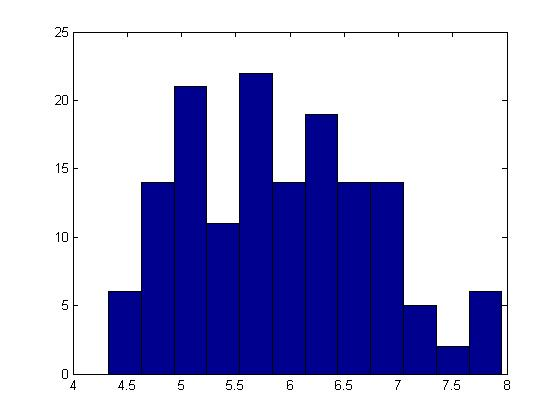
\includegraphics[width=.22\textwidth]{\figdir/hw1_3_1} &
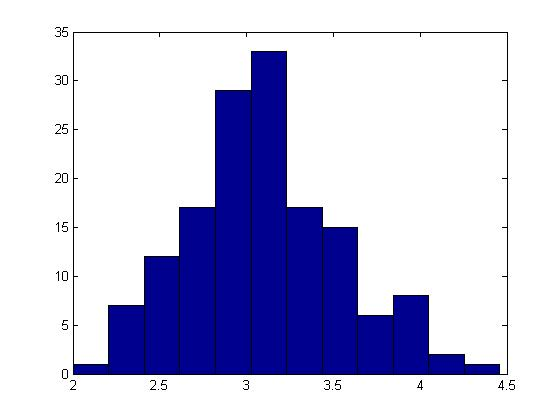
\includegraphics[width=.22\textwidth]{\figdir/hw1_3_2} &
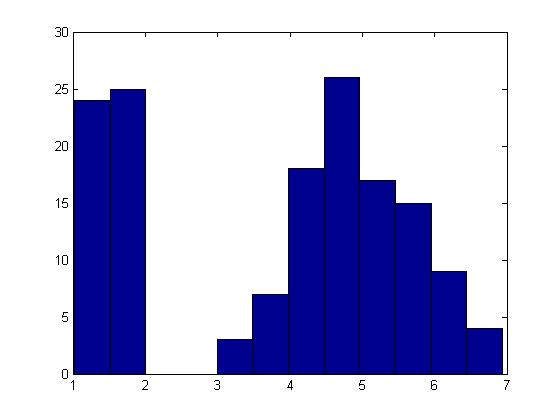
\includegraphics[width=.22\textwidth]{\figdir/hw1_3_3} &
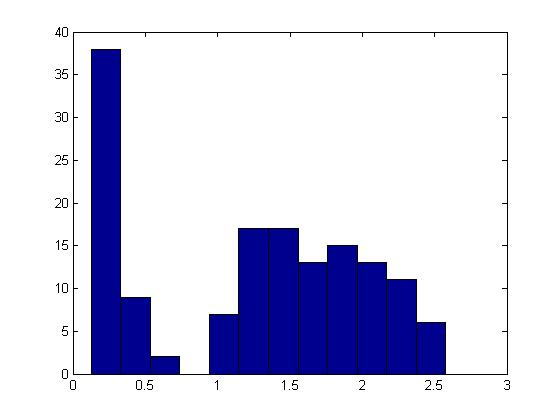
\includegraphics[width=.22\textwidth]{\figdir/hw1_3_4} \\
hist(X(:,1),12) & hist(X(:,2),12) & hist(X(:,3),12) & hist(X(:,4),12)
\end{tabular}
\end{figure}

\vspace{3ex}
\textbf{(c) Compute the mean of the data points for each feature (mean)}

\textit{MEAN(X)} is a row vector containing the mean value of each column. So I use \textit{MEAN(X)} to calculate average or mean value for each feature:  5.9001, 3.0989, 3.8196, 1.2526

\vspace{3ex}
\textbf{(d) Compute the variance and standard deviation of the data points for each feature}

\textit{VAR(X)} returns the variance of the values in \textit{X}, and \textit{STD(X)} returns the standard deviation. The standard deviation is the square root of variance.

So the variance of the data points for each feature is 0.6993, 0.1916, 3.0976, 0.5797, and the standard deviation of the data points for each feature is 0.8362, 0.4378, 1.7600, 0.7613.

NOTE: 

\textit{VAR(X)} and \textit{STD(X)} use the default normalization by \textit{N-1}, where \textit{N} is the sample size. 

\textit{VAR(X,1)} and \textit{STD(X,1)} normalizes by \textit{N}, \textit{VAR(X,0)} and \textit{STD(X,0)} is the same as \textit{STD(X)}.

\vspace{3ex}
\textbf{(e) "Normalize" the data by subtracting the mean value from each feature, and dividing by its
standard deviation. (This will make the data zero-mean and unit variance.) Show your code.
Note: you can do this with a for-loop (easy, but slow in Matlab), or in a "vectorized" form
using repmat or bsxfun (faster, but harder to read).}

Normalization, \textit{X$_{norm}$ = $\frac{X-\mu}{\sigma}$}, means adjusting values measured on different scales to a notionally common scale, and this will make the data zero-mean and unit variance.


\textit{ZSCORE(X)} returns a centered, scaled version of \textit{X}

Also, I can get the same solution using following code:
\begin{lstlisting}
 x=X(:,1);   % the first feature of X
 xnorm=(x-repmat(mean(x), length(x), 1)) / std(x);    % normalization
\end{lstlisting}
\vspace{3ex}
\textbf{(f) For each pair of features (1,2), (1,3), and (1,4), plot a scatterplot ("plot") of the feature
values, colored according to their target value (class). (For example, plot all data points with
y = 0 as blue, y = 1 as green, etc.) You may find the commands "find" and "hold on" useful
for this. Alternatively, the command "scatter" may be useful.}

Taking the pair of features (1,2) as an example:

\begin{lstlisting}
 scatter(X(:,1),X(:,2),[],Y,'filled');
\end{lstlisting}

Also, I can get the same solution using following code:

\begin{lstlisting}
 hold on;
 scatter(x(find(iris(:,end) == 0),1),x(find(iris(:,end) == 0),2),'.','r');
 scatter(x(find(iris(:,end) == 1),1),x(find(iris(:,end) == 1),2),'.','b');
 scatter(x(find(iris(:,end) == 2),1),x(find(iris(:,end) == 2),2),'.','g');
\end{lstlisting}

\begin{figure}[h!] \centering
\begin{tabular}{cccc}
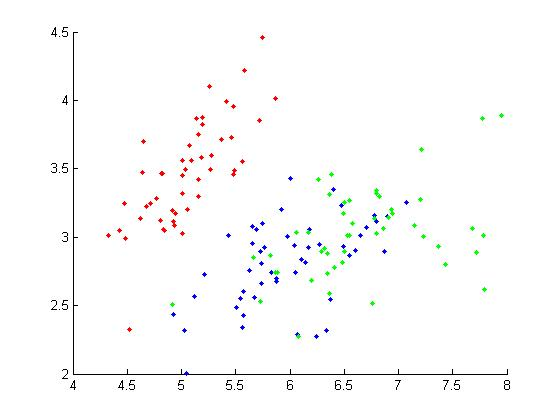
\includegraphics[width=.31\textwidth]{\figdir/hw1_3_5} &
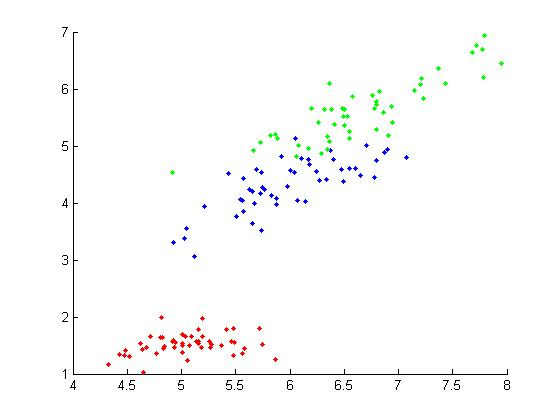
\includegraphics[width=.31\textwidth]{\figdir/hw1_3_6} &
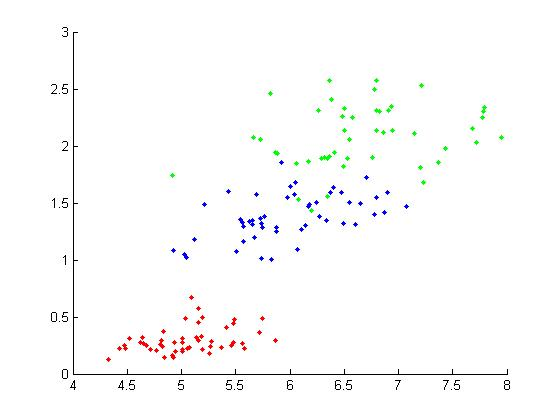
\includegraphics[width=.31\textwidth]{\figdir/hw1_3_7} \\
Features (1,2) & Features (1,3) & Features (1,4)
\end{tabular}
\end{figure}

\subsection*{Problem 4: Plotting functions}
To plot a function in Matlab, you simply choose a selection of x locations, compute their associated
y values, and plot it as a set of data points connected by lines.

\vspace{3ex}
\textbf{(a) Plot feature 1 (x-axis) versus feature 3 (y-axis).}
\begin{lstlisting}
 scatter(X(:,1),X(:,3),25,'r','filled');
\end{lstlisting}

\vspace{3ex}
\textbf{(b) To get the x and y range values, use ax=axis()}

\textit{ax=AXIS()} returns a row vector containing the scaling for the current plot. If the current view is 2-D, \textit{ax} has four components: [\textit{XMIN}, \textit{XMAX}, \textit{YMIN}, \textit{YMAX}].

Here \textit{ax} = 4, 8, 1, 7 
       
\vspace{3ex}
\textbf{(c) Create a collection of densely-spaced x points, e.g., xv = xmin:.01:xmax;}

According to the above question, \textit{xmin}=4 and \textit{xmax}=8.
\begin{lstlisting}
 xv = xmin:.01:xmax; % create a collection of densely-spaced x points
\end{lstlisting}
Then \textit{xv} is a collection of x points on the x-axis. Regression function, \textit{yv}, would be calculated based on these x points. 

\vspace{3ex}

\textbf{(d) Evaluate your function at each of these points, e.g., yv = 1.5 * (xv - 3);}

Calculate \textit{yv}. The regression function is y=1.5 * (x - 3):
\begin{lstlisting}
 yv = 1.5 * (xv - 3); % evaluate your function at each of these points
\end{lstlisting}

\vspace{3ex}

\textbf{(e) Plot this line in blue on top of your data points. To make the line thicker, you may want to
use options, "linethickness", 3, in your plot call.}

Firstly, use \textit{HOLD ON} to hold the current plot and all axis properties so that subsequent graphing commands add to the existing graph.

Secondly, plot the regression line with following command:

\begin{lstlisting}
 hold on;
 plot(xv,yv,'LineWidth',3,'Color','b');   % use option "LineWidth" to set thickness
\end{lstlisting}

\begin{figure}[h!] \centering
\begin{tabular}{cccc}
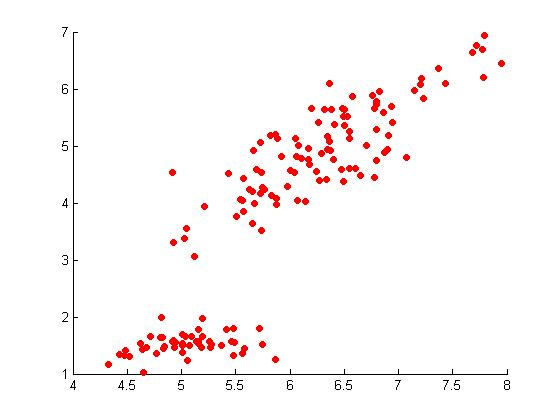
\includegraphics[width=.31\textwidth]{\figdir/hw1_4_1} &
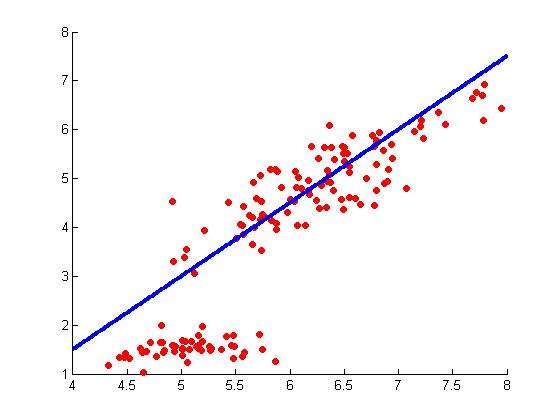
\includegraphics[width=.31\textwidth]{\figdir/hw1_4_2} \\
Feature 1 (x-axis) vs feature 3 (y-axis) & Line yv on top of the data points
\end{tabular}
\end{figure}


\subsection*{Problem 5: Writing a function}
Write a function dist that calculates the vector of Euclidean distances between a single vector \textit{x}
and a collection of data points (stored in a matrix) \textit{X}, e.g.,

$$ D_j = \sqrt{\sum\limits_{s}(x_{i}-X_{ji})^2} \qquad \forall j $$

\vspace{3ex}
Here is my implementation of function \textit{dist(x,X)}:
\begin{lstlisting}
 % calculate the distances of points from point x
 function D = dist(x,X)
    D=sqrt(sum((repmat(x,length(X),1)-X).^2,2)); 
 end;
\end{lstlisting}

\vspace{3ex}
Call the function \textit{dist(x,X)} to calculate the distances of the Iris data points from the first point, \textit{X(1,:)}:
\begin{lstlisting}
 % calculate the distances of the Iris data points from the first point in 4-D space
 dist(X(1,:),X);
\end{lstlisting}

Then \textit{D} = [0; 0.2889; 0.3310; 0.6050; 1.0828; ... 5.2303; 4.7107; 4.2405; 4.4869; 4.6512] (the first five numbers in D and the last five numbers in D)

\vspace{3ex}
Show a histogram of the distances of the Iris data points from the first point:
\begin{lstlisting}
 hist(dist(X(1,:),X),12);
\end{lstlisting}

\begin{figure}[h!] \centering
\begin{tabular}{cccc}
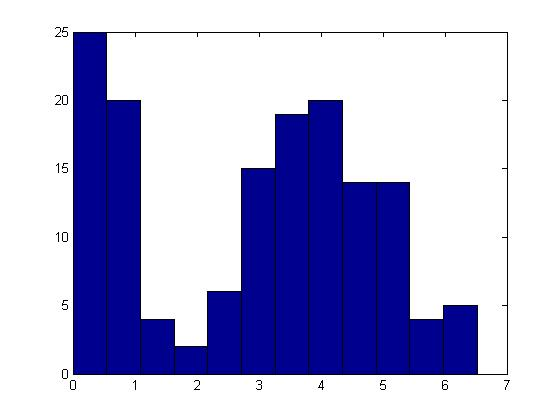
\includegraphics[width=.50\textwidth]{\figdir/hw1_5_1} \\ hist(dist(X(1,:),X),12)
\end{tabular}
\end{figure}

\end{document}
